%Dies ist die Hauptseite des Dokumentes. Es werden u. a. alle Kapitel,
%Einstellung im Header eingebunden.  Veränderungen müssen in folgenden Dateien
%vorgenommen werden:
      %- Layout.tex
      %- newComments.tex
      %- Titelseite
      %- Versionsübersicht
      %- einzelne Kapitel (evtl. erweitern)


% Definition von globalen Parametern, die derzeit auf der Titelseite und in der
% Kopfzeile verwendet werden. Der in <> gesetzte Text ist zu verändern.

\newcommand{\praktikumTitel}{WiReLib}
\newcommand{\projektTitel}{WiReLib}


%Hier sind alle Einstellungen enthalten, die sich auf das Seiten- und
%Dokumentenlayout beziehen

\documentclass[
  11pt,                % Schriftgröße
  DIV12,
  german,              % für Umlaute, Silbentrennung etc.
  oneside,            % einseitiges Dokument
  titlepage,          % es wird eine Titelseite verwendet
  parskip=half,        % Abstand zwischen Absätzen (halbe Zeile)
  headings=normal,      % Größe der Überschriften verkleinern
  captions=tableheading,  % Beschriftung von Tabellen unterhalb ausgeben
  final                % Status des Dokuments (final/draft)
]{scrreprt}            %


%------Ändern von Schriftschnitten - (Muss ganz am Anfang stehen !) ------------
\usepackage{fix-cm}

%------Umlaute -----------------------------------------------------------------
%   Umlaute/Sonderzeichen wie äüöß können direkt im Quelltext verwenden werden.
%    Erlaubt automatische Trennung von Worten mit Umlauten.
\usepackage[T1]{fontenc}
\usepackage[utf8]{inputenc}

%------Anpassung der Landessprache----------------------------------------------
\usepackage{ngerman}

%------Einfache Definition der Zeilenabstände und Seitenränder------------------
\usepackage{geometry}
\usepackage{setspace}
\usepackage{xspace}

%------Schriftgrößenanpassung von einzelnen Textpassagen------------------------
\usepackage{relsize}

%------Trennlinien in Kopf- und Fusszeile
\usepackage[headsepline, footsepline, ilines]{scrpage2}

%------Grafiken-----------------------------------------------------------------
\usepackage{graphicx}

%------Packet zum Sperren, Unterstreichen und Hervorheben von Texten------------
\usepackage{soul}

%------ergänzende Schriftart----------------------------------------------------
\usepackage{helvet}

%------Lange Tabellen-----------------------------------------------------------
\usepackage{longtable}
\usepackage{array}
\usepackage{ragged2e}
\usepackage{lscape}

%------PDF-Optionen-------------------------------------------------------------
\usepackage[
  bookmarks,
  bookmarksopen=true,
  colorlinks=true,
  linkcolor=black,        % einfache interne Verknüpfungen
  anchorcolor=black,      % Ankertext
  citecolor=black,        % Verweise auf Literaturverzeichniseinträge im Text
  filecolor=black,        % Verknüpfungen, die lokale Dateien öffnen
  menucolor=black,        % Acrobat-Menüpunkte
  urlcolor=black,         % Farbe für URL-Links
  backref,                % Zurücktext nach jedem Bibliografie-Eintrag als
                          % Liste von Überschriftsnummern
  pagebackref,            % Zurücktext nach jedem Bibliografie-Eintrag als
                          % Liste von Seitenzahlen
  plainpages=false,       % zur korrekten Erstellung der Bookmarks
  pdfpagelabels,          % zur korrekten Erstellung der Bookmarks
  hypertexnames=false,    % zur korrekten Erstellung der Bookmarks
  linktocpage             % Seitenzahlen anstatt Text im Inhaltsverzeichnis
                          % verlinken
  ]{hyperref}

%-----Glossar-Optionen----------------------------------------------------------
\usepackage{translator}
\usepackage[				   %
acronym,		% ein Abkürzungsverzeichnis erzeugen
toc,			% Taucht im Inhaltsverzeichnis auf
]				   
{glossaries}
\makeglossaries

\usepackage{xcolor}
\definecolor{lightergray}{rgb}{0.9,0.9,0.9}

\usepackage{listings}
\lstset{numbers=left, numberstyle=\tiny, numbersep=5pt,
breaklines=true, backgroundcolor=\color{lightergray},
basicstyle=\ttfamily,
}
\usepackage{booktabs}
      % enthält eingebundene Packete

%------Seitenränder-------------------------------------------------------------
\geometry{verbose,                     % zeigt die eingestellten Parameter beim
                                       % Latexlauf an
      paper=a4paper,                   % Papierformat
      top=25mm,                        % Rand oben
      left=25mm,                       % Rand links
      right=25mm,                      % Rand rechts
      bottom=45mm,                     % Rand unten
      pdftex                           % schreibt das Papierformat in die
                                       % Ausgabe damit Ausgabeprogramm
                                       % Papiergröße erkennt
  }

%Seitenlayout
\onehalfspace        % 1,5-facher Abstand

%------Kopf- und Fußzeilen -----------------------------------------------------
\pagestyle{scrheadings}

%------Kopf- und Fußzeile auch auf Kapitelanfangsseiten ------------------------
\renewcommand*{\chapterpagestyle}{scrheadings}

%------Schriftform der Kopfzeile -----------------------------------------------
\renewcommand{\headfont}{\normalfont}

%------Kopfzeile----------------------------------------------------------------
\setlength{\headheight}{21mm}        % Höhe der Kopfzeile
\ihead{\large{\textsc{\praktikumTitel}}\\    % Text in der linken Box
       \small{\projektTitel}}
\chead{}                            % Text in der mittleren Box

%----Fusszeile
\cfoot{}                            % Text in mittlerer Box
\ofoot{\pagemark}                    % Seitenzahl in rechter Box
           % Diese Datei enthält alle
                                           % Layouteinstellungen

%------Beginn des Gesamtdokumentes----------------------------------------------
\begin{document}

%------Eingebundene Seiten, Verzeichnisse bzw. Kapitel--------------------------
% Dies ist die Titelseite des Grobentwurfs.
% Die in "<...>" sind zu ersetzen
% Die Ausgabe darf 1 Seite nicht überschreiten, also ggf. Abstände anpassen
% Die Angabe in [...] gibt den Abstand nach der entsprechenden Zeile an.


%----Stil dieser Seite----------------------------------------------------------
\thispagestyle{plain}      % Kopfzeile bleibt leer

%----Beginn der Titelseite------------------------------------------------------
\begin{titlepage}

%----zentrierte Ausrichtung über die gesamte Seite----------------------------
\begin{center}

%----Titel des Praktikum (\praktikumTitel in newComments zu verändern)--------
{\relsize{4}{\textbf{\textsc{\praktikumTitel}}}}\\[3ex]%[5ex]

%----Titel des Teilprojektes (\projektTitel in newComments verändern)---------
{\relsize{3}{\textbf{\textsc{\projektTitel}}}}\\[3ex]%[5ex]

Software-Entwicklungspraktikum (SEP)\\
Sommersemester 2012\\[4ex]%[6ex]

{\relsize{3}\so{\textbf{Grobentwurf}}}\\[4ex]%[5ex]

%----eingebundenes Logo der TU--------------------------------------------------

\includegraphics[scale=0.8]{bilder/carolo.jpg}\\[4ex]%[5ex]

%----Daten des Auftraggebers
Auftraggeber\\
Technische Universität Braunschweig\\
Wissenschaftliches Rechnen\\
Prof. Hermann G. Matthies\\
Hans-Sommer-Straße 65\\
D-38092 Braunschweig\\[1ex]%[2ex]
Betreuer: Elmar Zander\\[4ex]%[5ex]

% ----Tabelle der Praktikumsteilnehmer------------------------------------------
Auftragnehmer:
\begin{tabular}{l<{\hspace{20mm}} l<{\hspace{30mm}}}\\
  Name                   &   E-Mail-Adresse\\      % Zeilenüberschift
  \hline                    % Linie unterhalb der Zeilenüberschrift
  %----Nachfolgend alle Namen und E-Mail-Adressen der Teilnehmer einfügen
  Eric Anders 		& eric.anders89@web.de\\
  Johann Hong 		& johann.hong@googlemail.com\\
  Jörn Hameyer 		& j.hameyer@tu-bs.de\\
  Marco Melzer 		& marco.melzer@tu-braunschweig.de\\
  Markus Dietrich 	& markus.dietrich@tu-bs.de\\
  Philipp Offensand & PhilippOffensand@gmx.de\\
  Stephan Sobol 	& stephan.sobol@web.de\\
  Theodor van Nahl 	& t.nahl@tu-bs.de
\end{tabular}\\[1ex]%[2ex]

Braunschweig, 24.04.2012

\end{center}
\end{titlepage}

                       % Titelseite
%Diese Datei dient der Versionskontrolle. Sie ist vollständig zu bearbeiten.

%----Überschrift------------------------------------------------------------
{\relsize{2}\textbf{Versionsübersicht}}\\[2ex]

%----Start der Tabelle------------------------------------------------------
\begin{longtable}{|m{1.78cm}|m{1.59cm}|m{2.86cm}|m{1.9cm}|m{5.25cm}|}

  \hline                                              % Linie oberhalb

  %----Spaltenüberschriften------------------------------------------------
  \textbf{Version}  &    \textbf{Datum}  &    \textbf{Autor}  &
  \textbf{Status}   &    \textbf{Kommentar}       \\  %Spaltenüberschrift
  \hline                                              % Gitterlinie

  %----die nachfolgeden beiden Zeilen so oft wiederholen und die ... mit den
  %    entsprechenden Daten zu füllen wie erforderlich
  0.1   &    16.05.2012    &    Theodor van-Nahl    &   in Bearbeitung     &    Analyse der Produktfunktionen F100-F200\\       % Eintrag in Zeile
  \hline                                              % Gitterlinie unten
  0.2   &    17.05.2012    &    Jörn Hameyer    &   in Bearbeitung     &    Analyse der Produktfunktionen F226-F229\\       % Eintrag in Zeile
  \hline
  0.3   &    18.05.2012    &    Stephan Sobol    &   in Bearbeitung     &    Analyse der Produktfunktionen F220-F225\\       % Eintrag in Zeile
  \hline
  0.4   &    18.05.2012    &    Philipp \mbox{Offensand}    &   in Bearbeitung     &    Qualitätsanalyse\\       % Eintrag in Zeile
  \hline
  0.5   &    18.05.2012    &    Markus Dietrich    &   in Bearbeitung     &    Analyse der Produktfunktionen F230-F302\\       % Eintrag in Zeile
  \hline
  0.6   &    18.05.2012    &    Johann Hong    &   in Bearbeitung     &    Analyse der Produktfunktionen F210-F214\\       % Eintrag in Zeile
  \hline
  0.7   &    18.05.2012    &    Marco Melzer    &   in Bearbeitung     &    Einleitung\\       % Eintrag in Zeile
  \hline
  0.8   &    18.05.2012    &    Philipp \mbox{Offensand}    &   in Bearbeitung     &    Komponentenspezifikation\\       % Eintrag in Zeile
  \hline
  0.9   &    19.05.2012    &    Theodor van-Nahl    &   in Bearbeitung     &    Analyse der Produktfunktion F201-F210\\       % Eintrag in Zeile
  \hline
  0.10   &   21.05.2012    &    Marco Melzer    &   in Bearbeitung     &    Schnittstellenspezifikation\\       % Eintrag in Zeile
  \hline
  0.11   &   22.05.2012    &    Joahann Hong    &   in Bearbeitung     &    Verteilungsentwurf\\       % Eintrag in Zeile
  \hline
  0.12   &   23.05.2012    &    Jörn Hameyer,\newline Stephan Sobol    &   in Bearbeitung     &    Protokolle für die Benutzung der Komponenten\\       % Eintrag in Zeile
  \hline
  1.0   &    23.05.2012    &    sämtliche Auftragnehmer    &   abgenommen     &    \\       % Eintrag in Zeile
  \hline
  

%----Ende der Tabelle------------------------------------------------------
\end{longtable}

Status: "`in Bearbeitung"' oder "`abgenommen"'
Kommentar: hier eintragen, was ge\"andert bzw. ergänzt wurde


Hinweis zum Template:
Dieses Template enth\"ult Hinweise, die alle kursiv geschrieben sind. Alles
Kursivgeschriebene ist selbstverst\"andlich bei Abgabe zu entfernen sind.
Angaben in <\ldots> sind mit dem entsprechendem Text zu f\"ullen.  \"Uberz\"ahlige
Kapitel, d.h. Kapitel, die nicht bearbeitet werden m\"ussen, da sie nicht der
Aufgabenstellung entsprechen, bitte entfernen.

Aufgabe des Grobentwurfs: Aufgabe dieses Dokumentes ist es, die Architektur des
Systems zu beschreiben und die daraus resultierenden Pakete durch die
Definition von Schnittstellen zu Komponenten auszubauen.
        % Versionsübersicht

\tableofcontents                           % Inhaltsverzeichnis wird automatisch
                                           % generiert
\listoffigures                             % ebenso das Abbildungsverzeichnis

%----Kapitel des Feinentwurfs, die mit Inhalt zu füllen sind--------------------
% Kapitel 1
% Die Unterkapitel können auch in separaten Dateien stehen,
% die dann mit dem \include-Befehl eingebunden werden.
%-------------------------------------------------------------------------------

\chapter{Zielbestimmung}

%Hier Einleitungstext einfügen, dabei die Formatierungen selber erstellen
Dieser Abschnitt hat die Aufgabe, als eine Art Einleitung zu dienen. Es soll
ein kurzer Umriss über Ziel und Motivation des Gesamt- und ggf. der
Teilprojekte dargestellt werden. Beschrieben wird die Hauptaufgabe des Systems.
Wichtig ist, den Grund für die Systementwicklung (Probleme oder Geschäftsidee)
und damit ihre Ziele herauszuarbeiten.
\section{Musskriterien}

Hier wird aufgeführt, welche Funktionalitäten/Leistungen das Softwareprodukt in
jedem Fall erfüllen muss, damit es genutzt werden kann.
\section{Wunschkriterien}
Dies sind Kriterien, die für die Lauffähigkeit des Produkts nicht zwingend
erforderlich sind, für die Erreichung der Projektziele aber erfüllt werden
sollten.

\section{Abgrenzungskriterien}
Hier ist zu verdeutlichen, welche Ziele mit dem Produkt bewusst nicht erreicht
werden sollen oder werden können.
            % Kapitel 1
% Kapitel 2 mit den entsprechenden Unterkapiteln
% Die Unterkapitel können auch in separaten Dateien stehen,
% die dann mit dem \include-Befehl eingebunden werden.
%------------------------------------------------------------------------------------
\chapter{Produkteinsatz}
Das Produkt soll als neues System f"ur die Bibliotheksverwaltung in die Institut-Homepage f"ur "`Wissenschaftliches Rechnen"' (http://www.wire.tu-bs.de) integriert werden, und dabei das alte Vorhandene ersetzen. Die Zielgruppe des Produktes beschr"ankt sich dabei nicht nur auf die Mitarbeiter des Institutes, sondern schliesst aufgrund eines Webinterfaces auch Mitglieder der TU Braunschweig oder einfachen Nutzern der Institutsseite mit ein. 
In den folgenden Punkten werden die voraussichtlichen Anwendungsbereiche, die Zielgruppen und die Betriebsbedingungen explizit aufgef"uhrt. 

\section{Anwendungsbereiche}
Das Produkt dient als Managementsystem im "`Bibliothek"'-Bereich des Institutes.

\section{Zielgruppen}
Zielgruppen sind die Mitarbeiter des Institutes, Studenten der TU Braunschweig, Nutzer der \gls{UB} und diverse Nutzer der Institutshomepage.

\section{Betriebsbedingungen}
Aufgrund der Nutzerfreundlichkeit eines universell genutzten Bibliothekssystems, soll 
f"ur den Betrieb ein Notebook oder ein einfacher Desktop PC ausreichen. Das Produkt soll mit allen g"angigen Betriebssystemen (Windows (XP/Vista/7), Unix/Linux) kompatibel sein und ebenso keine Schwierigkeiten mit verbreiteten Browsern wie Mozilla Firefox, Internet Explorer, etc.\ haben. Der Webserver für das Produkt sollte mit g"angigen Linuxdistributionen (mit Linux-Kernel 3.0+) kompatibel sein.             % Kapitel 2
% Kapitel 3
%-------------------------------------------------------------------------------
\chapter{Produktübersicht}

\begin{figure}[h]
\centering
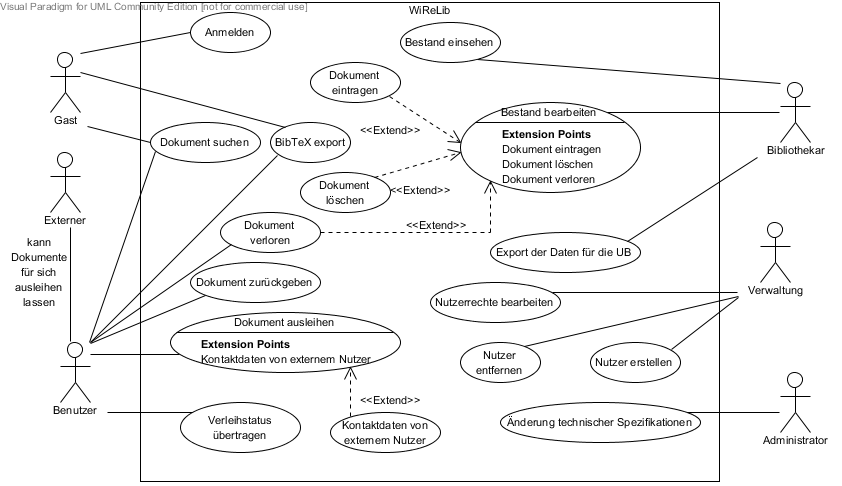
\includegraphics[width=0.8\linewidth]{bilder/use-case.png}
\caption[Use-Case-Diagramm]{Use-Case-Diagramm}
\label{use-case}
\end{figure}

Beschreibung des \nameref{use-case}es:

Benutzer, die nicht angemeldet sind, werden als Gäste geführt.
Gäste können sich anmelden und sind dann Nutzer.
Auch können Gäste Dokumente suchen und herausfinden, ob sie vorhanden sind, oder ob sie bereits verliehen wurden.

Ein Nutzer darf wie ein Gast nach Dokumenten suchen.
Zusätzlich darf er Dokumente ausleihen und muss diese auch wieder zurückgeben.
Wenn ihm ein Dokument verloren geht, sollte er dies melden.
Auch darf ein Nutzer ein ausgeliehenes Dokument weitergeben.
Dabei wird der Verleihstatus auf die andere Person übertragen.
Wenn dies \gls{glos:ext}\ sind, so müssen die Kontaktdaten hinterlegt werden.

Der Bibliothekar kann den Bestand der Dokumente einsehen und ihn bearbeiten.
Das heißt, dass er neue Dokumente eintragen kann, aus der Suchoption entfernen, oder ein Dokument als verloren markieren, sodass, falls möglich, neu bestellt werden kann.
Der Bibliothekar kann durch einen Button eine Datei exportieren, welche für die \gls{UB} lesbar ist.
Somit kann auch von der \gls{UB} aus ein gesuchtes Dokument gefunden werden.

Die Verwaltung darf Nutzer erstellen, Nutzerrechte bearbeiten und gegebenenfalls Nutzer entfernen.

Der Administrator hat vollen Zugriff auf das System und kann alle technische Spezifikationen vornehmen.
         % Kapitel 3
% Kapitel 4
%-------------------------------------------------------------------------------

\chapter{Produktfunktionen}

\section{Allgemeine Funktionen}
\subsection{F100 (Anmeldung)}
\label{F:Anmeldung}
\begin{description}
  \item[Geschäftsprozess]Anmeldung
  \item[Ziel]Ein Benutzer meldet sich erfolgreich am System an.
  \item[Vorbedingung]Der Benutzer ist bereits auf dem System registriert und besitzt ein Passwort.
  \item[Nachbedingung Erfolg]Der Benutzer findet sich auf seiner Benutzerseite wieder.
  \item[Nachbedingung Fehlschlag]Das Passwort wurde falsch eingegeben. Der Benutzer erhält eine Meldung, dass der Benutzer oder das Passwort falsch eingegeben wurden.
  \item[Akteure]Gast/Benutzer
  \item[Auslösendes Ereignis]Der Benutzer erhält die Möglichkeiten, sich Dokumente zu leihen oder den Status geliehener Dokumente zu ändern.
  \item[Beschreibung]\hfill
    \begin{enumerate}
      \item Der Benutzer wählt den Link \emph{Login} auf der Webseite aus.
      \item Der Benutzer gibt seinen Nutzernamen und sein Passwort ein.
      \item Der Benutzer bestätigt seine Eingaben.
      \item Das System prüft die Korrektheit der Eingaben.
      \item Das System leitet den Benutzer entsprechend der Korrektheit seiner Daten weiter.
    \end{enumerate}
\end{description}

\subsection{\emph{optional:} F101 (Anmeldung über LDAP)}
\label{F:AnmeldungAFS}
\begin{description}
  \item[Geschäftsprozess]Anmeldung eines Institusnutzers.
  \item[Ziel]Ein Benutzer meldet sich über seinen \gls{GITZ}-Account am System an.
  \item[Vorbedingung]Der Benutzer besitzt einen \gls{LDAP}-Account, ist auf dem System registiert und hat ein gültiges Passwort.
  \item[Nachbedingung Erfolg]Der Benutzer findet sich auf einer persönlichen Benutzerseite wieder.
  \item[Nachbedingung Fehlschlag]Der Benutzer bekommt eine Fehlermeldung.
  \item[Akteure]Gast/Benutzer
  \item[Auslösendes Ereignis]Der Benutzer erhält die Möglichkeiten, sich Dokumente zu leihen oder den Status geliehener Dokumente zu ändern.
  \item[Beschreibung]\hfill
    \begin{enumerate}
      \item Der Benutzer wählt den Link \emph{Login} auf der Webseite aus.
      \item Der Benutzer gibt seinen Nutzernamen und sein Passwort ein.
      \item Der Benutzer bestätigt seine Eingaben.
      \item Das System prüft die Korrektheit der Eingaben, indem sie über das \gls{LDAP}-System der TU Braunschweig validiert werden.
      \item Das System leitet den Benutzer entsprechend der Korrektheit seiner Daten weiter.
    \end{enumerate}
\end{description}

\subsection{F102 (Anbindung an die Universitätsbibliothek)}
\begin{description}
  \item[Geschäftsprozess]Übertragung der Institutsbibliothek an die \gls{UB}.
  \item[Ziel]Angleichung der im \gls{UB}-\gls{glos:Allegro} verfügbaren Daten über die Institutsbibliothek.
  \item[Vorbedingung]Keine.
  \item[Nachbedingung Erfolg]Der Benutzer erhält eine Datei mit den Daten im \gls{glos:Allegro}-Format, die er an die \gls{UB} per Mail verschicken kann.
  \item[Nachbedingung Fehlschlag]Das System soll die Export-Funktion nur berechtigten Benutzern bieten, damit soll ein Fehlschlag in der Bedienung abgefangen werden. Sollte der Vorgang des Parsens einen Fehler erzeugen (z.\,B. durch eine gesperrte Datenbank), erhält der Benutzer die Bitte, es später noch einmal zu versuchen.
  \item[Akteure]Bibliothekar
  \item[Beschreibung]\hfill
    \begin{enumerate}
      \item Der Benutzer fordert über das Webinterface die \gls{glos:Allegro}-Datei an.
      \item Das System überträgt die Dokumente der Datenbank in das \gls{glos:Allegro}-Format.
      \item Das System gibt dem Benutzer eine Datei zum Download, die der Benutzer manuell an die \gls{UB} versenden kann.
    \end{enumerate}
  \item[Erweiterung]\hfill
    \begin{itemize}
      \item \emph{optional} Das System übernimmt das Versenden der E-Mail.
    \end{itemize}
  \item[Alternativen]
\end{description}

\subsection{F103 (Mailtexte ändern)}
\begin{description}
  \item[Geschäftsprozess]Der Administrator passt den Text für generierte E-Mails an.
  \item[Ziel]Vom System generierte E-Mails sind leicht anpassbar.
  \item[Vorbedingung]Keine.
  \item[Nachbedingung Erfolg]E-Mails der geänderten Klasse werden mit dem neuen Text verschickt.
  \item[Nachbedingung Fehlschlag]Der Administrator bekommt eine Meldung vom System zum Fehler.
  \item[Akteure]Administrator
  \item[Beschreibung]\hfill
    \begin{enumerate}
      \item Der Administrator geht auf eine Seite des Systems, die ihm allgemeine Einstellungen ermöglicht.
      \item Der Administrator ändert den Text der gewünschten E-Mail.
      \item Der Administrator bestätigt seine Änderung.
    \end{enumerate}
  \item[Erweiterungen]
  \item[Alternativen]
\end{description}


\section{Dokumentfunktionen}
Die Dokumentfunktionen beschreiben jeden direkten Umgang mit der durch das System verwalteten Dokumente. Darunter ist die \emph{Einpflege} (F200-F202), \emph{Suche} (F210-F219), \emph{Ausleihe} (F220-F229) und der Export (F230-F239).
\subsection{F200 (Bib\TeX-Import)}
\begin{description}
  \item[Geschäftsprozess]Dokumente hinzufügen mit \BibTeX.
  \item[Ziel]Neu in die Bibliothek aufgenommene Dokumente in die Verwaltung aufnehmen und zur Ausleihe verfügbar machen.
  \item[Vorbedingung]Der Benutzer hat sich bereits erfolgreich angemeldet und hat die Rolle \emph{Bibliothekar}. Der Benutzer ist im Besitz einer \BibTeX -Datei mit mindestens einem eingetragenen Dokument.
  \item[Nachbedingung Erfolg]Das neue Dokument befindet sich im System (inkl. Eintrag in der Datenbank) und besitzt entweder den Status \emph{verfügbar} oder \emph{bestellt}.
  \item[Nachbedingung Fehlschlag]Der Benutzer erhält eine Meldung zum Fehlschlag und den Hinweis die \BibTeX -Datei zu überprüfen. Es findet kein Eintrag in die Datenbank statt.
  \item[Akteure]Bibliothekar
  \item[Auslösendes Ereignis]Der Benutzer bekommt eine Übersicht zu neu eingetragenen Dokumenten.
  \item[Beschreibung]\hfill
    \begin{enumerate}
      \item Der Benutzer befindet sich auf der Seite zur \BibTeX einpflege.
      \item Der Benutzer wählt eine \BibTeX -Datei von seinem Rechner.
      \item Der Benutzer wählt den späteren Status, der in den Dokumenten vermerkt sein soll.
      \item Der Benutzer startet einen Upload in das System.
      \item Das System prüft die Datei auf Validität. Dabei ist vor allem zu beachten, dass \TeX-Umlaute und -Sonderzeichen in ein \gls{glos:unicode} Format übersetzt werden und die Einträge valides \gls{glos:unicode} sind.
	(Validität schließt sowohl den \BibTeX -Umfang ein, wie auch die Felder: \emph{DateOfPurchase}, \emph{price}, \emph{InventarNo}, \emph{InformatikBibNo}, \emph{LibraryOfCongressNo}, \emph{CIPNo}, \emph{XtraNo}, \emph{keywords}.) Umlaute und Sonderzeichen können auch direkt in \gls{glos:unicode} angegeben werden.
	Das System prüft ebenfalls, ob ein entsprechender Eintrag bereits vorhanden ist.
      \item Das System trägt die Dokumente in die Datenbank ein.
      \item Das System fügt den Dokumenten den vom Benutzer bestimmten Status hinzu.
      \item Das System macht die Daten verfügbar.
      \item Das System leitet den Benutzer zu einer Übersicht weiter.
    \end{enumerate}
  \item[Erweiterung]Der Benutzer hat die Möglichkeit, nicht vorher spezifizierte Felder in die \BibTeX -Datei einzutragen.
  \item[Alternativen]Der Benutzer registriert das Dokument über ein reines Webinterface.
\end{description}

\subsection{F201 (Webinterface-Import)}
\label{F:Web-Import}
\begin{description}
  \item[Geschäftsprozess]Dokument hinzufügen über das Webinterface.
  \item[Ziel]Ein neu in die Bibliothek aufgenommenes Dokument in die Verwaltung aufnehmen und zur Ausleihe verfügbar machen.
  \item[Vorbedingung]Der Benutzer hat sich bereits erfolgreich angemeldet und hat die Rolle \emph{Bibliothekar}. Der Benutzer ist im Besitz aller Daten, die zur Eintragung des Dokumentes erforderlich ist.
  \item[Nachbedingung Erfolg]Das neue Dokument befindet sich im System (inkl. Eintrag in der Datenbank) und besitzt entweder den Status \emph{verfügbar} oder \emph{bestellt}.
  \item[Nachbedingung Fehlschlag]Der Benutzer erhält eine Meldung zum Fehlschlag und den Hinweis, die eingegebenen Daten zu prüfen. Es findet kein Eintrag in die Datenbank statt.
  \item[Akteure]Bibliothekar
  \item[Auslösendes Ereignis]Der Benutzer bekommt eine Übersicht zum neu eingetragenen Dokument.
  \item[Beschreibung]\hfill
    \begin{enumerate}
      \item Der Benutzer befindet sich auf der Seite zur Einpflege über das Webinterface.
      \item Der Benutzer wählt den Typ des Dokumentes und erhält alle Eingabefelder, die für dieses Dokument notwendig und optional sind. Das System stellt die Basisfelder, die in \BibTeX\ zur Verfügung stehen, wie auch die Felder: \emph{DateOfPurchase}, \emph{price}, \emph{InventarNo}, \emph{InformatikBibNo}, \emph{LibraryOfCongressNo}, \emph{CIPNo}, \emph{XtraNo}, \emph{keywords}.
      \item Der Benutzer bestätigt seine Eingaben.
      \item Das System prüft die Eingaben auf Validität und vorhandene Einträge.
      \item Das System trägt das Dokument in die Datenbank ein.
      \item Das System fügt den Dokumenteneintrag den vom Benutzer bestimmten Status hinzu.
      \item Das System macht die Daten verfügbar.
      \item Das System leitet den Benutzer zu einer Übersicht weiter.
    \end{enumerate}
    %% TODO:
  \item[Erweiterung]Der Benutzer hat die Möglichkeit, nicht vorher spezifizierte Felder selbst einzufügen.
  \item[Alternativen]Der Benutzer registriert das Dokument über den \BibTeX Import.
\end{description}

\subsection{F202 (Editieren von Dokumenten)}
\begin{description}
  \item[Geschäftsprozess]Der Eintrag eines Dokumentes wird verändert.
  \item[Ziel]siehe oben.
  \item[Vorbedingung]Das Dokument existiert im System.
  \item[Nachbedingung Erfolg]Die Änderungen waren zulässig und werden in die Datenbank übernommen.
  \item[Nachbedingung Fehlschlag]Die Änderungen waren nicht zulässig und der Benutzer wird auf den Eingabefehler aufmerksam gemacht.
  \item[Akteure]Bibliothekar
  \item[Beschreibung]\hfill
    \begin{enumerate}
      \item Der Benutzer wählt die Option \emph{Dokument editieren}
      \item Das System leitet den Benutzer an eine Seite ähnlich zu \nameref{F:Web-Import}.
      \item Der Benutzer führt seine Anpassungen durch und bestätigt.
      \item Das System übernimmt die Anpassungen.
    \end{enumerate}
  \item[Erweiterung]
  \item[Alternativen]
\end{description}

\subsection{\emph{optional:} F203 (Löschen von Dokumenten)}
\label{F:Löschen}
\begin{description}
  \item[Geschäftsprozess]Das Löschen eines Dokumentes aus dem System.
  \item[Ziel]Das Dokument wird vollständig aus dem System entfernt, wie auch alle im Bezug stehenden Daten.
  \item[Vorbedingung]Das Dokument ist als \emph{vermisst} markiert.
  \item[Nachbedingung Erfolg]Keine Information zu dem Dokument existiert mehr im System.
  \item[Nachbedingung Fehlschlag]Der Fehler wird abgefangen und die Datenbank wird nicht verändert.
  \item[Akteure]Administrator
  \item[Beschreibung]\hfill
    \begin{enumerate}
      \item Der Administrator wählt auf der Dokumentenseite die Option \emph{Dokument löschen}.
      \item Das System bittet den Administrator um Bestätigung.
      \item Der Administrator bestätigt den Löschvorgang.
      \item Das System entfernt alle Datenbankeinträge, die zu dem Dokument gehören.
    \end{enumerate}
  \item[Erweiterung]
  \item[Alternativen]
\end{description}

\subsection{F210 (Generelle Suche)}
\label{F:Suche}
\begin{description}
  \item[Geschäftsprozess]Der Benutzer sucht im System einen bestimmten Dokumenteneintrag.
  \item[Ziel]Der Benutzer bekommt alle seiner Suche entsprechenden Einträge.
  \item[Vorbedingung]Der Benutzer befindet sich auf der Seite mit der Suchmaske.
  \item[Nachbedingung Erfolg]Der Benutzer bekommt eine Liste aller Suchergebnisse.
  \item[Nachbedingung Fehlschlag]Es konnte kein Dokument der Suche entsprechend gefunden werden. Es wird ein Hinweis ausgegeben.
  \item[Akteure]Gast oder Benutzer
  \item[Auslösendes Ereignis]Die Suche wird gespeichert, um später darauf wieder zurückgreifen zu können.
  \item[Beschreibung]\hfill
    \begin{enumerate}
      \item Der Benutzer gibt seine Suchwörter ein. Dabei kann der Benutzer mehrere Worte verwenden, die entsprechend in den Dokumenteneinträgen enthalten sind (Die Reihenfolge ist nicht relevant). Mehrere Wörter werden automatisch logisch mit \emph{und} verknüpft.
      \item Der Benutzer bestätigt seine Eingabe.
      \item Das System durchsucht seine Datenbank, um Dokumenteneinträge mit den eingegebenen Teilworten zu finden.
      \item Das System gibt eine Seite zurück, die alle passenden Einträge anzeigt.
    \end{enumerate}
    \item[Erweiterung]Erweiterungen der Suche sind \nameref{F:extSuche}, \nameref{F:n00bSuche} und \nameref{F:regexSuche}
\end{description}


\subsection{F211 (Suche mit erweiterten Ausdrücken)}
\label{F:extSuche}
\begin{description}
  \item[Geschäftsprozess]Der Benutzer kann bei der Suche Teilworte verwenden.
  \item[Ziel]Der Benutzer kann komplexe Mittel verwenden, um nach möglichen Zeichenfolgen zu suchen.
  \item[Vorbedingung]Der Benutzer befindet sich auf der Seite mit der Suchmaske.
  \item[Nachbedingung Erfolg]Der Benutzer bekommt eine Liste aller Suchergebnisse.
  \item[Nachbedingung Fehlschlag]Es konnte kein Dokument der Suche entsprechend gefunden werden. Dem Benutzer wird ein Hinweis zurück gegeben.
  \item[Akteure]Gast oder Benutzer
  \item[Auslösendes Ereignis]Die Suche wird gespeichert, um später darauf wieder zurück greifen zu können.
  \item[Beschreibung]\hfill
    \begin{enumerate}
      \item Der Benutzer gibt seine Ausdruck ein. 
	\begin{itemize}
	  \item Einzelne Ausdrücke werden durch ein Leerzeichen getrennt, um der Trennung zu entgehen, müssen die Ausdrücke mit einfachen oder doppelten Hochkommata zu einem Ausdruck zusammen gefasst werden. 
	  \item Mehrere Ausdrücke können mit \emph{AND} und \emph{OR} oder mit \emph{UND} und \emph{ODER} verknüpft werden.
	  \item Bestimmte Felder können direkt angesprochen werden, darunter Titel und Autor. Angesprochen werden die Felder mit z.\,B. „title:``Tim und Struppi''“.
	\end{itemize}
      \item Der Benutzer bestätigt seine Eingabe.
      \item Das System durchsucht seine Datenbank, um Dokumenteneinträge mit den eingegebenen Teilworten zu finden.
      \item Das System gibt eine Seite zurück, die alle passenden Einträge anzeigt, wie auch den Suchterm des Benutzers.
    \end{enumerate}
\end{description}

\subsection{\emph{optional:} F212 (erweiterte Suche)}
\label{F:n00bSuche}
\begin{description}
  \item[Geschäftsprozess]Der Benutzer sucht ein Dokument.
  \item[Ziel]Eine vereinfachte Suchmaske ermöglicht allen Benutzern die Nutzung von erweiterten Ausdrücken.
  \item[Vorbedingung]Der Benutzer befindet sich auf der Seite mit der erweiterten Suchmaske.
  \item[Nachbedingung Erfolg]Der Benutzer bekommt eine Liste aller Suchergebnisse.
  \item[Nachbedingung Fehlschlag]Es konnte kein Dokument der Suche entsprechend gefunden werden.
  \item[Akteure]Gast oder Benutzer
  \item[Auslösendes Ereignis]Die Suche wird gespeichert, um später darauf wieder zurückgreifen zu können.
  \item[Beschreibung]\hfill
    \begin{enumerate}
      \item Der Benutzer öffnet die Maske für die erweiterte Suche.
      \item Das System stellt dem Benutzer extra Felder, die ihm die Möglichkeiten von \nameref{F:extSuche} ermöglichen, ohne die Kommandos zu kennen.
      \item Der Benutzer bestätigt die eingetragenen Parameter.
      \item Das System gibt dem Benutzer die Liste mit den Suchergebnissen zurück, wie auch den Suchterm des Benutzers.
    \end{enumerate}
\end{description}


\subsection{\emph{optional:} F213 (Suche mit regulären Ausdrücken)}
\label{F:regexSuche}
\begin{description}
  \item[Geschäftsprozess]Der Benutzer kann bei der Suche \gls{glos:regex}  verwenden.
  \item[Ziel]Der Benutzer kann komplexe Mittel verwenden, um nach möglichen Zeichenfolgen zu suchen.
  \item[Vorbedingung]Der Benutzer befindet sich auf einer extra Seite für eine erweiterte Suche.
  \item[Nachbedingung Erfolg]Der Benutzer bekommt eine Liste aller Suchergebnisse.
  \item[Nachbedingung Fehlschlag]Es konnte kein Dokument der Suche entsprechend gefunden werden oder es wurde keine validen \gls{glos:regex} angegeben. Es wird ein Hinweis ausgegeben.
  \item[Akteure]Gast oder Benutzer
  \item[Auslösendes Ereignis]Die Suche wird gespeichert, um später darauf wieder zurückgreifen zu können.
  \item[Beschreibung]\hfill
    \begin{enumerate}
      \item Der Benutzer gibt seine \gls{glos:regex} ein, die für die Suche verwendet werden sollen. Mehrere \gls{glos:regex} müssen eventuell mit \emph{AND}, \emph{OR}, \emph{UND} oder \emph{ODER} getrennt werden.
      \item Der Benutzer bestätigt seine Eingabe.
      \item Das System durchsucht seine Datenbank, um Dokumenteneinträge mit den eingegebenen Teilworten zu finden.
      \item Das System gibt eine Seite zurück, die alle passenden Einträge anzeigt, wie auch den Suchterm des Benutzers.
    \end{enumerate}
\end{description}

\subsection{F214 (Sortierung der Suche)}
\begin{description}
  \item[Geschäftsprozess]Der Benutzer ordnet sein Suchergebnis nach gewünschter Spalte.
  \item[Ziel]Das System ordnet das Suchergebnis.
  \item[Vorbedingung]Der Benutzer hat bereits seine Suchergebnisse.
  \item[Nachbedingung Erfolg]Das Ergebnis wird nach der vom Benutzer gewünschten Spalte sortiert.
  \item[Nachbedingung Fehlschlag]Dieser Fall sollte im System nicht möglich sein.
  \item[Akteure]Gast oder Benutzer
  \item[Auslösendes Ereignis]Aktualisierung der Seite.
  \item[Beschreibung]\hfill
    \begin{enumerate}
      \item Der Benutzer klickt auf die gekennzeichnete Spaltenüberschrift.
      \item Lokal wird ihm die Suche aktualisiert.
    \end{enumerate}
\end{description}

\subsection{F220 (Ausleihe)}
\begin{description}
  \item[Geschäftsprozess]Der Benutzer entnimmt ein Dokument der Bibliothek.
  \item[Ziel]Es gibt eine Übersicht für andere Benutzer, welche Bücher verfügbar sind. Es gibt auch eine Übersicht, welches Dokument der Benutzer selbst ausgeliehen hat.
  \item[Vorbedingung]Der Benutzer ist im System registiert und angemeldet.
  \item[Nachbedingung Erfolg]Der Benutzer kann ein Dokument der Bibliothek entnehmen, da es im System registriert ist.
  \item[Nachbedingung Fehlschlag]Das Buch ist wahrscheinlich derzeit nicht verfügbar, der Benutzer muss es später nocheinmal versuchen.
  \item[Akteure]Benutzer
  \item[Auslösendes Ereignis]Das Dokument ändert ihren Status von \emph{verfügbar} auf \emph{verliehen}. Der Benutzer sieht bei diesem Dokument einen Hinweis, dass er sie ausgeliehen hat, zusätzlich zu einer persönlichen Ausleihliste.
  \item[Beschreibung]\hfill
    \begin{enumerate}
      \item Der Benutzer sucht das gewünschte Dokument über die Systemsuche.
      \item Der Benutzer befindet sich auf der Detail-Ansicht des Dokumentes.
      \item Wenn das Dokument verfügbar ist, wählt der Benutzer die Option \emph{ausleihen}.
      \item Das System ändert den Status des Dokumentes auf \emph{verliehen} und registriert den Benutzer entsprechend.
    \end{enumerate}
\end{description}

\subsection{F221 (Ausleihe an Externe)}
\begin{description}
  \item[Geschäftsprozess]Der \gls{glos:ext} leiht sich ein Dokument.
  \item[Ziel]Der Benutzer kann sich das Dokument für die Dauer der Leihfrist mitnehmen.
  \item[Vorbedingung]Der Benutzer hat einen \emph{Benutzer} als Bürgen und das Dokument ist verfügbar.
  \item[Nachbedingung Erfolg]Der Benutzer kann das Dokument der Bibliothek entnehmen und sowohl auf der Liste der geliehenen Dokumente des Bürgen, wie auch auch auf der Seite des Dokumentes findet sich der Name des  Benutzers. Auf der Seite des Dokumentes ist weiter der Name des Bürgen zu entnehmen.
  \item[Nachbedingung Fehlschlag]Das Buch ist wahrscheinlich derzeit nicht verfügbar, der Benutzer muss es später nocheinmal versuchen.
  \item[Akteure]Der \gls{glos:ext} und ein Benutzer 
  \item[Beschreibung]\hfill
    \begin{enumerate}
      \item Der Benutzer bittet einen \emph{Benutzer} als Bürgen, für ihn das Dokument zu entleihen.
      \item Der Bürge wählt das Dokument aus und wählt dort die Option \emph{leihen für externe Person}.
      \item Der Bürge trägt die Personalien (Name, E-Mail und Adresse) sowie die Dauer der Leihfrist ein.
      \item Der Bürge bestätigt und das System trägt die Daten in die Datenbank ein.
    \end{enumerate}
  \item[Erweiterung]
  \item[Alternativen]
\end{description}

\subsection{F222 (Ausleihe übertragen)}
\begin{description}
  \item[Geschäftsprozess]Ein Benutzer $A$ gibt ein Dokument an eine an einen anderen Benutzer $B$ weiter.
  \item[Ziel]Der Benutzer $A$ registiert einen anderen Benutzer $B$ als Leihender.
  \item[Vorbedingung]Der Benutzer $A$ ist derzeit Leihender des Dokumentes.
  \item[Nachbedingung Erfolg]Der Benutzer $B$ ist Leihender des Dokumentes.
  \item[Nachbedingung Fehlschlag]Der Benutzer $A$ bleibt Leihender des Dokumentes, es wird nichts an der Datenbank geändert.
  \item[Akteure]Leihender Benutzer und zukünftig leihender Benutzer.
  \item[Beschreibung]\hfill
    \begin{enumerate}
      \item Der Benutzer $A$ wählt das Dokument aus.
      \item Der Benutzer $A$ wählt die Option \emph{übertragen} aus.
      \item Der Benutzer $A$ gibt Benutzer $B$ ein.
      \item Das System ändert die Ausleihe auf Benutzer $B$.
    \end{enumerate}
  \item[Erweiterung]
  \item[Alternativen]Der Benutzer $B$  überträgt das Dokument von Benutzer $A$ auf sich.
\end{description}

\subsection{F223 (Ausleihe zurückgeben)}
\begin{description}
  \item[Geschäftsprozess]Der Benutzer bringt ein Dokument zurück in die Bibliothek.
  \item[Ziel]Das Dokument ist wieder \emph{verfügbar}.
  \item[Vorbedingung]Der Benutzer ist Leihender des Dokumentes.
  \item[Nachbedingung Erfolg]Der Benutzer ist nicht mehr Leihender des Dokumentes und die Literatur ist wieder \emph{verfügbar}.
  \item[Nachbedingung Fehlschlag]Der Benutzer wird über den Fehler informiert und wird gebeten, es später erneut zu versuchen.
  \item[Akteure]Benutzer
  \item[Beschreibung]\hfill
    \begin{enumerate}
      \item Der Benutzer wählt das Dokument aus.
      \item Der Benutzer wählt auf der Dokumentenseite die Rückgabe aus.
      \item Das System ändert den Status des Dokumentes und verschiebt den Benutzer in die History der Leihenden.
    \end{enumerate}
  \item[Erweiterung]\gls{glos:ext} können ihr Buch an jede Person zurück geben und von denen entsprechend als Zurückgegeben markieren lassen.
  \item[Alternativen]
\end{description}

\subsection{\emph{optional:} F224 (Ausleihe vermisst melden)}
\begin{description}
  \item[Geschäftsprozess]Ein Dokument, das nicht mehr auffindbar ist, wird als \emph{vermisst} gemeldet.
  \item[Ziel]Alle Personen, die zum wieder Auffinden des Dokumentes beitragen könnten, werden Informiert.
  \item[Vorbedingung]Der Benuzter hat geprüft, ob das Dokument sich an dem Ort befindet, bei dem es auffindbar sein soll.
  \item[Nachbedingung Erfolg]Ein Benutzer, der das Dokument gesichtet hat, meldet sich per E-Mail.
  \item[Nachbedingung Fehlschlag]Der Bibliothekar bestellt das Buch nach und/oder meldet es als \emph{verloren} (Siehe \nameref{F:AusleiheVerlohren}).
  \item[Akteure]zwei Benutzer und ein Bibliothekar.
  \item[Beschreibung]\hfill
    \begin{enumerate}
      \item Der Benutzer stellt fest, dass das Dokument nicht, wie im System beschrieben, auffindbar ist.
      \item Der Benutzer wählt die Detailseite des Dokumentes aus.
      \item Der Benutzer wählt die Option \emph{vermisst melden}.
      \item Das System verschickt eine E-Mail mit den entsprechenden Informationen an eine Mailingliste für alle Benutzer.
    \end{enumerate}
  \item[Erweiterung]
  \item[Alternativen]Das System verschickt keine E-Mail, sondern meldet den Verlust über eine entsprechende Stelle auf dem System.
\end{description}

\subsection{F225 (Ausleihe verloren melden)}
\label{F:AusleiheVerlohren}
\begin{description}
  \item[Geschäftsprozess]Ein Dokument, das ausgeliehen wurde oder als verfügbar gilt, wird als verloren gemeldet.
  \item[Ziel]Nicht mehr auffindbare Dokumente können allgemein als vermisst gemeldet werden.
  \item[Vorbedingung]Das Dokument ist bereits im System registriert.
  \item[Nachbedingung Erfolg]Das Dokument gilt offiziell als vermisst.
  \item[Nachbedingung Fehlschlag]Der Fehler wird vom System an den Benutzer gemeldet.
  \item[Akteure]Bibliothekar
  \item[Beschreibung]\hfill
    \begin{enumerate}
      \item Der Benutzer befindet sich auf der Detailseite des Dokumentes
      \item Der Benutzer wählt eine Option \emph{verlohren melden}.
      \item Das System registriert den Vorgang.
      \item Das System schließt das Dokument in Zukunft bei normalen Suchen aus.
    \end{enumerate}
  \item[Erweiterung]\hfill
  \item[Alternativen]
\end{description}


\subsection{F226 (Ausleihfrist abgelaufen)}
\begin{description}
  \item[Geschäftsprozess]Die Leihfrist eines Dokumentes ist abgelaufen.
  \item[Ziel]Sowohl der Bürge als auch die Person, die das Dokument geliehen hat, werden per E-Mail noch einmal erinnert.
  \item[Vorbedingung]Die Person hat das Dokument geliehen und die Leihfrist ist abgelaufen.
  \item[Nachbedingung Erfolg]Beide Parteien sind via E-Mail nocheinmal erinnert worden.
  \item[Nachbedingung Fehlschlag]\hfill
    \begin{itemize}
      \item Die E-Mails konnten nicht verschickt werden, der Administrator wird benachrichtigt.
      \item Die E-Mail an die Person, die das Dokument geliehen hat, ist nicht korrekt oder konnte nicht zugestellt werden. Damit wird der Bürge benachrichtigt.
    \end{itemize}
  \item[Akteure]Das System
  \item[Beschreibung]\hfill
    \begin{enumerate}
      \item Das System prüft täglich ob eine Leihfrist abgelaufen ist.
      \item Das System stellt fest, dass eine Leihfrist abgelaufen ist.
      \item Das System sendet an beide Parteien eine E-Mail mit den Informationen, auch zu dem Dokument selbst.
    
    \end{enumerate}
  \item[Erweiterung]
  \item[Alternativen]
\end{description}

\subsection{F227 (Ausleihhistory)}
\begin{description}
  \item[Geschäftsprozess]Prüfung, wer das Dokument bereits ausgeliehen hat.
  \item[Ziel]Die Benutzer bekommen Einsicht in die Liste der Personen die dieses Dokument bereits ausgeliehen haben.
  \item[Vorbedingung]Das Dokument ist im System eingetragen und der Benutzer ist am System angemeldet.
  \item[Nachbedingung Erfolg]Das Dokument wurde bereits ausgeliehen, daher bekommt der Benutzer die Liste.
  \item[Nachbedingung Fehlschlag]Das Dokument wurde noch nicht ausgeliehen oder es gab einen anderen Fehler, in beiden Fällen wird das dem Benutzer gemeldet.
  \item[Akteure]Bibliothekar
  \item[Beschreibung]\hfill
    \begin{enumerate}
      \item Der Benutzer befindet sich auf der Dokumentenansicht.
      \item Das System stellt dem Benutzer eine Liste mit der Ausleihhistory.
    \end{enumerate}
  \item[Erweiterung]
  \item[Alternativen]
\end{description}

\subsection{F228 (Derzeitiger Leihender)}    %TODO
\begin{description}
  \item[Geschäftsprozess]Leihenden abrufen.
  \item[Ziel]Ein Benutzer, der dieses Recht besitzt, kann bei verliehenen Büchern sehen, an wen das Buch verliehen ist.
  \item[Vorbedingung]Das gewählte Dokument ist verliehen und der Benutzer verfügt über ausreichend Rechte.
  \item[Nachbedingung Erfolg]Der Benutzer bekommt den derzeitig Ausleihenden angezeigt.
  \item[Nachbedingung Fehlschlag]Der Leihstatus konnte nicht abgerufen werden.
  \item[Akteure]Benutzer 
  \item[Beschreibung]\hfill
  \begin{enumerate}
  \item Benutzer wählt gewünschtes Dokument aus.
  \item Der derzeitig Ausleihende angezeigt.
  \end{enumerate}
  \item[Erweiterung]
  \item[Alternativen]
\end{description}

\subsection{F229 (Entleihliste)}
\begin{description}
  \item[Geschäftsprozess]Vom Benutzer geliehene Dokumente.
  \item[Ziel]Der Benutzer sieht die Dokumente, die er selbst geliehen hat und für die er gebürgt hat, ein.
  \item[Vorbedingung]Der Benutzer ist im System angemeldet.
  \item[Nachbedingung Erfolg]Der Benutzer erhält eine Liste über alle Dokumente, die er geliehen hat und für die er gebürgt hat.
  \item[Nachbedingung Fehlschlag]Der Benutzer wird über den enstandenen Fehler informiert.
  \item[Akteure]Benutzer
  \item[Beschreibung]\hfill
    \begin{enumerate}
      \item Der Benutzer wählt seine persönliche Seite über die Entleihe aus.
      \item Das System gibt die beschriebene Seite dem Benutzer zurück.
    \end{enumerate}
  \item[Erweiterung]
  \item[Alternativen]
\end{description}

\subsection{F230 (Bib\TeX -Export)}
\begin{description}
  \item[Geschäftsprozess]Dokumentinformationen für \BibTeX-Einbindung herunterladen.
  \item[Ziel]Der Benutzer erhält alle notwendigen Informationen zu einem Buch im \BibTeX-Format, um diese z.\,B. in ein eigenes Dokument ein zu binden.
  \item[Vorbedingung]Der Benutzer befindet sich auf der Detailsseite des Dokumentes.
  \item[Nachbedingung Erfolg]Der Benutzer erhält den Code für \BibTeX .
  \item[Nachbedingung Fehlschlag]Der Benutzer wird von dem System über den Fehler informiert.
  \item[Akteure]Gast oder Benutzer
  \item[Beschreibung]\hfill
    \begin{enumerate}
      \item Der Benutzer wählt die Detailseite des gewünschten Dokumentes aus.
      \item Das System bietet dem Benutzer einen Link \emph{\BibTeX}, der vom Benutzer ausgewählt wird.
      \item Das System gibt dem Benutzer die entsprechenden \BibTeX -Informationen zurück.
    \end{enumerate}
  \item[Erweiterung]
  \item[Alternativen]
\end{description}

\subsection{F231 (Universitätsbibliothek-Export)}
\begin{description}
  \item[Geschäftsprozess]Export zur \gls{UB}.
  \item[Ziel]Die gewählten Dokumente werden an die \gls{UB} übermittelt.
  \item[Vorbedingung]Der Ausführender Benutzer hat genügend Rechte.
  \item[Nachbedingung Erfolg]Der Benutzer hat eine Datei für den Versand an die \gls{UB}.
  \item[Nachbedingung Fehlschlag]Die Datei konnte nicht erzeugt werden, der Benutzer erhält vom System eine Fehlermeldung.
  \item[Akteure]Bibliothekar
  \item[Beschreibung]Die gewählten Dokumente werden in das \gls{glos:Allegro}-Format der \gls{UB} konvertiert und übermittelt.
  \item[Erweiterung]
  \item[Alternativen]
\end{description}


\section{Benutzer und System}
Im Folgenden werden die Funktionalitäten zu den Benutzerrollen, Benutzern und der Administration beschrieben.

\subsection{F301 (Benutzerverwaltung)}
\begin{description}
  \item[Geschäftsprozess]Benutzerverwaltung und -Erzeugung.
  \item[Ziel]Benutzer werden angelegt und verwaltet.
  \item[Vorbedingung]Ausführender Benutzer hat ausreichend Rechte.
  \item[Nachbedingung Erfolg]Benutzer wurde erfolgreich bearbeitet.
  \item[Nachbedingung Fehlschlag]Änderungen wurden nicht übernommen, das System informiert über den aufgetretenen Fehler.
  \item[Akteure]Verwalter oder Administrator.
  \item[Beschreibung]Registrierte Benutzer werden über eine Weboberfläche erstellt, Rollen zugewiesen (siehe \nameref{F:rollen}) und gelöscht.
  \item[Erweiterung]
  \item[Alternativen]
\end{description}

\subsection{F302 (Rechtezuweisung für Rollen)} 
\begin{description}
  \item[Geschäftsprozess]Eine Benutzerrolle bekommt ein oder mehrere Rechte zugewiesen.
  \item[Ziel]Eine Benutzerrolle kann nachträglich im Umfang erweitert oder eingeschränkt werden.
  \item[Vorbedingung]Ändernder Nutzer hat ausreichende Rechte.
  \item[Nachbedingung Erfolg]Die Rolle hat neue Rechte bekommen und/oder alte Rechte verloren.
  \item[Nachbedingung Fehlschlag]Die Rechte wurden nicht übernommen.
  \item[Akteure]Verwalter oder Administrator.
  \item[Beschreibung]\hfill
  \begin{enumerate}
  \item Administrator oder Verwalter wählt zu ändernde Rolle aus.
  \item Zugeteilte Rechte werden angepasst.
  \item \emph{optional:} Nutzer mit der entsprechenden Rolle bekommen eine E-Mail zugeschickt mit dem Hinweis auf die Änderung.
  \end{enumerate}
  \item[Erweiterung]
  \item[Alternativen]
\end{description}

\subsection{F303 (Benutzer Rolle(n) zuweisen)}
\label{F:rollen}
\begin{description}
  \item[Geschäftsprozess]Der Benutzer mit entsprechenden Rechten verteilen Rollen an andere Benutzer.
  \item[Ziel]Ein Benutzer bekommt eine Rolle zugeteilt von einem Administrator oder einem Benutzerverwalter.
  \item[Vorbedingung]Der ändernde Benutzer hat ausreichende Rechte.
  \item[Nachbedingung Erfolg]Der zu ändernde Benutzer hat eine neue Rolle zugewiesen bekommen.
  \item[Nachbedingung Fehlschlag]Der zu ändernde Benutzer hat die Rolle nicht gewechselt.
  \item[Akteure]Verwalter oder Administrator.
  \item[Beschreibung]\hfill
  \begin{enumerate}
  \item Administrator oder Benutzerverwalter wählt zu ändernden Benutzer aus.
  \item Eine neue Rolle wird eingetragen.
  \item \emph{optional:} Der geänderte Nutzer bekommt eine E-Mail zugeschickt mit dem Hinweis auf die Änderung.
  \end{enumerate}
  \item[Erweiterung]
  \item[Alternativen]
\end{description}
         % Kapitel 4
% Kapitel 5
%------------------------------------------------------------------------------------------

\chapter{Produktdaten}
/D10/ Daten über einen Nutzer:
\begin{itemize}
  \item Daten werden von der Verwaltung eingegeben.
  \item Bestandteile:
  \begin{itemize}
    \item[*] User:
    \begin{itemize}
      \item[-] Username
      \item[-] Passwort, falls ohne AFS gearbeitet wird
      \item[-] Vorname
      \item[-] Nachname
      \item[-] E-Mail
      \item[-] Adresse
      \item[-] Telefon
      \item[-] Rolle
    \end{itemize}
    \item[*] Externe:
    \begin{itemize}
      \item[-] dasselbe wie beim User bis auf den Usernamen und die Rolle
    \end{itemize}
  \end{itemize}
\end{itemize}

\newpage

/D20/ Daten über Dokumente:
\begin{itemize}
  \item Dateneingabe erfolgt über den Bibliothekar.
  \item Löschen eines Dokumentes aus der Datenbank ist allgemein nicht möglich.
  \item Bestandteile:
  \begin{itemize}
    \item[*] ID
    \item[*] Titel
    \item[*] Autoren
    \item[*] ISBN
    \item[*] Kategorie
    \item[*] Status (0 = vorhanden, 1 = ausgeliehen, 2 = bestellt, 3 = vermisst, 4 = verloren gegangen)
    \item[*] weitere Eingaben möglich
  \end{itemize}
\end{itemize}

/D30/ Verleihdaten
\begin{itemize}
  \item Zu jedem Dokument wird eine Verleihhistorie erstellt.
  \item Die Daten können nicht gelöscht werden. Sie werden lediglich bei weiteren Verleihungen erweitert.
  \item Bestandteile:
  \begin{itemize}
    \item[*] Ausleihdatum
    \item[*] Rückgabedatum
    \item[*] Entleihfrist
    \item[*] Entleiher
    \item[*] evtl. einen Externen
    \item[*] das Dokument
  \end{itemize}
\end{itemize}              % Kapitel 4
% Kapitel 6
%-------------------------------------------------------------------------------

\chapter{Nichtfunktionale Anforderungen}


%----Start der Tabelle------------------------------------------------------
\begin{tabular}{|c|c|c|c|c|}
  \hline                                              % Linie oberhalb

  %----Spaltenüberschriften------------------------------------------------
  \textbf{Produktqualität}  & \textbf{sehr gut}  &    \textbf{gut}  &
  \textbf{normal}           & \textbf{nicht relevant}  \\  %Spaltenüberschrift
  \hline                                              % Gitterlinie

  %----die nachfolgeden beiden Zeilen so oft wiederholen und die ... mit den
  %    entsprechenden Daten zu füllen wie erforderlich
Funktionalität  &x&&&\\        % Eintrag in Zeile
  \hline
Angemessenheit&&x&&\\
\hline
Richtigkeit&&x&&\\
\hline
Interoperabilität&&x&&\\
\hline
Ordnungsmäßgkeit&&x&&\\
\hline
Sicherheit&&x&&\\
\hline
Zuverlässigkeit&&x&&\\
\hline
Reife&x&&&\\
\hline
Fehlertoleranz&&&x&\\
\hline
Wiederherstellbarkeit&&x&&\\
\hline
Benutzbarkeit&x&&&\\
\hline
Verständlichkeit&x&&&\\
\hline
Erlernbarkeit&x&&&\\
\hline
Bedienbarkeit&x&&&\\
\hline
Effizienz&&&x&\\
\hline
Zeitverhalten&&&x&\\
\hline
Verbrauchsverhalten&&x&&\\
\hline
Änderbarkeit&&x&&\\
\hline
Analysierbarkeit&&x&&\\
\hline
Modifizierbarkeit&x&&&\\
\hline
Stabilität&x&&&\\
\hline
Prüfbarkeit&&x&&\\
\hline
Übertragbarkeit&&&&x\\
\hline
Anpassbarkeit&&&x&\\
\hline
Installierbarkeit&&&&x\\
\hline
Konformität&&x&&\\
\hline
Austauschbarkeit&&&x&\\
\hline
%----Ende der Tabelle------------------------------------------------------
\end{tabular}


\section{Qualitätsmerkmale Sicherheit}
\subsection{/Q10/} Der Login über die Funktionen /\nameref{F:Anmeldung}/ und /\nameref{F:AnmeldungAFS}/ sowie Cookies sind verschlüsselt.
\subsection{/Q11/} SQL-Injections sollen bei der Suche von Dokumenten sowie bei anderen Eingaben nicht möglich sein. Dadurch sollen Sicherheitslücken vermieden werden.
\section{Qualitätsmerkmale Bedienbarkeit}
\subsection{/Q20/} Die Layoutstruktur und Fonts der Webseite sollen ähnlich sein denen des \Gls{glos:copdes} der TU Braunschweig. Dadurch soll die Webseite nicht aus dem einheitlichen Layout der TU Braunschweig herausfallen. Weiterhin soll damit eine weitere Anpassung an das \gls{CMS}\ der TU Braunschweig erleichtert werden.
\subsection{/Q21/} Das Layout der Webseite soll aufgeräumt sein mit klarer Navigation und Schaltflächen. Links sollen als solche markiert werden und nicht mit dem restlichen Text verschmelzen. Ebenso sollen auf der Webseite dargestellte Informationen wie \mbox{z.\,B.}\xspace Autor/Titel eines Dokumentes leicht ersichtlich und übersichtlich angezeigt werden.
\subsection{/Q22/} Die Bedienung der Funktionen /\nameref{F:Suche}/ und /\nameref{F:extSuche}/ soll intuitiv und einfach verständlich sein. Es soll kein tiefgehendes Wissen notwendig sein, um die Suche zu bedienen.
\section{Qualitätsmerkmale Sonstiges}
\subsection{/Q30/} Intern sollen alle Zeichenketten als \Gls{glos:unicode} bearbeitet werden. Damit werden Zeichensatzinkompatiblitäten vermieden und gleichzeitig alle Sonderzeichen ermöglicht.
\subsection{/Q31/} Nur als \emph{bestellt} markierte Dokumente dürfen mit der Funktion /\nameref{F:Löschen}/ gelöscht werden. Bereits vorhandene Dokumente dürfen nur als \emph{vermisst} beziehungsweise \emph{verloren} markiert werden. Optional: Administratoren dürfen auch bereits vorhandene Dokumente löschen.
        % Kapitel 4
\chapter{Benutzeroberfläche}

Grundlegend ist die Benutzeroberfläche in drei Web-Seiten unterteilt:
Zunächst die Anfangsseite, von der alle anderen Aktionen gestartet werden können.
Das Seitenlayout ist wie folgend geplant:


\section{/B10/ Seitenlayout}

 \begin{itemize}
   \item Bibliothek
   \begin{itemize}
    \item Suche
      \begin{description}
       \item[Einfache Suche] Die einfache Suche soll intuitiv funktionieren, sie besteht lediglich aus einer Eingabefläche, worin der Benutzer
       Dokumenttitel, Autoren oder Sonstiges eingeben kann. 
       \item[Erweiterte Suche] Die erweiterte Suche stellt dem anspruchsvolleren Anwender mehrere Eingabeflächen zur Verfügung, um gezielter suchen zu können 
       \end{description}
      \item Rückgabe
      \item (Eintragen)(nur vorhanden, falls als Bibliothekar eingeloggt; für weitere Informationen s. Nutzergruppen)
      \item Einloggen
    \end{itemize}
    \item Literaturverzeichnis
    \item Administration
 \end{itemize}
 
\begin{figure}
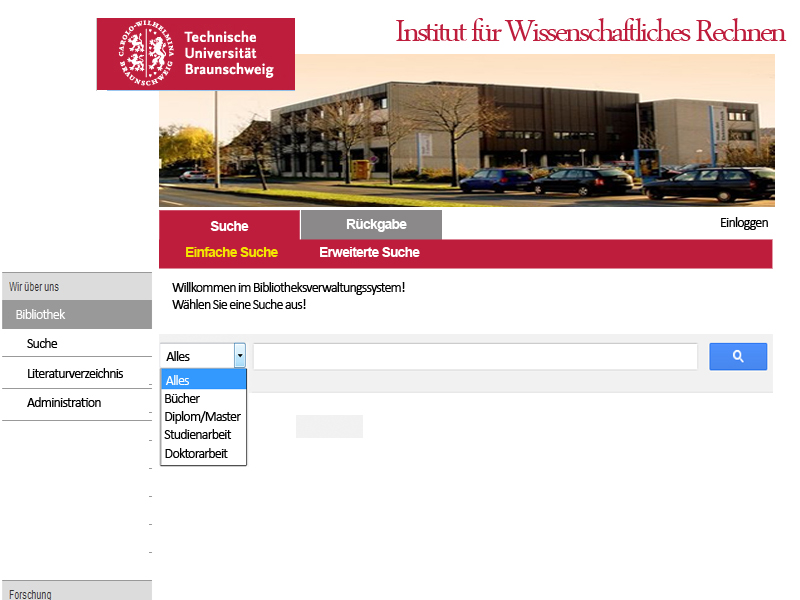
\includegraphics[width=0.8\linewidth]{bilder/layout2.jpg}
\caption{Beispiel für ein Seitenlayout}
\end{figure}

Suchergebnisse werden in einem großen Bereich rechts bzw. unter der Navigation angezeigt. Die Dokumente werden übersichtlich in tabellenartiger Form bereitgestellt. Bei einem Klick auf ein Dokument des Suchergebnisses erscheinen genauere Informationen über das Dokument (Titel,Autor,Jahr etc.), sowie
seinen Status (ausgeliehen, vorhanden, verloren).
Oben rechts wird zudem der eingeloggte User angezeigt.
Bei einem Klick auf den eingeloggten User ist eine Account-Verwaltungsseite geplant.



\section{/B20/ Account-Verwaltungsseite}
  	 	
Hier kann der Benutzer seinen Account verwalten, d.h. er/sie kann die persönlichen Daten und die E-Mail Adresse ändern.
Zusätzlich gibt es hier eine Liste alle Dokumente, welche der eingeloggte User zu eben diesem Zeitpunkt ausgeliehen hat.



\section{/B30/ Administration}

Nur der Administrator hat auf diese Schaltfläche Zugriff, bei allen anderen Nutzern mit weniger Rechten wird eine Fehlermeldung ausgegeben.
Hier kann der Administrator grundlegende Systemeinstellungen ändern und Benutzern Rechte zuweisen.



\section{/B40/ Nutzergruppen}

Darüber hinaus sind mehrere Nutzergruppen geplant(falls nicht anders angegeben, sind die Rechte vom Gast bis zum Administrator aufsteigend additiv zunehmend, d.h. ein Bibliothekar kann neue Dokumente einpflegen, ein Administrator kann dieses auch, aber hat zudem die Möglichkeit Rechte zuzuweisen etc.) 

\begin{description}
\item[Besucher] Wenn ein Nutzer unangemeldet die Seite betritt bzw. auf der Seite ist, gilt er als Besucher(Siehe Abbildung).
\item [\Gls{glos:ext}] Ein Externer ist ein Benutzer, welcher sich nicht anmelden kann. Er wird nur intern verwaltet und hat deswegen die gleiche Sicht
auf das Webinterface wie ein Besucher.
\item [Normaler Benutzer] Als normaler Benutzer gilt ein angemeldeter Benutzer ohne besondere Rechte. Er hat die Möglichkeit, sich Dokumente auszuleihen, und hat Zugriff auf seine eigene Account-Verwaltungsseite.
\item [Bibliothekar] Ein Bibliothekar hat erste Verwaltungsrechte. Ist ein Benutzer als Bibliothekar angemeldet, verändert sich die Navigation des Webinterfaces. Es erscheint zusätzlich eine Schaltfläche „Eintragen“, womit er/sie neue Dokumente in die Bibliothek einpflegen kann.
\item [Verwaltung] Ein Benutzer mit Verwaltungsrechten kann neue Benutzer anlegen und sie bearbeiten.
\item [Administrator] Der Administrator schließlich hat die Möglichkeit, über eine geplante erscheinende Schaltfläche „Administration“, Rechte zu verteilen, d.h. er kann zum Beispiel normalen Benutzern Verwaltungsrechte zuteilen oder entziehen. 
\end{description}











 
       % Kapitel 4
% Kapitel 10
% Die Unterkapitel können auch in separaten Dateien stehen,
% die dann mit dem \include-Befehl eingebunden werden.
%-------------------------------------------------------------------------------

\chapter{Technische Produktumgebung}

In diesem Kapitel wird die technische Umgebung des Produktes beschrieben. Bei
Client / Server  Anwendungen ist die Umgebung jeweils für Client und Server
getrennt anzugeben.

\section{Software}
\begin{itemize}
\item Server-Betriebssystem:              Linux
\item Client-Betriebssystem:                Browser
\item Frameworkprogramm :                Django
\item Programmiersprache:                  Python 2.6+
\item Zur Erstellung der Datenbank:   SQLite
\end{itemize}



\section{Hardware}
\begin{itemize}
\item Server: PC
\item Client: Computer
\end{itemize}

\section{Orgware}

Durch Internetverbindung zum WebsServer soll man sich über die Dokumente in der Bibliothek informieren können, und 
diese ausleihen oder je nach Rolle anderweitig verwalten. Die Verbindung zum Webserver wird per https  gesichert. 



\section{Produktschnittstellen}

Es wird folgende Schnittstellen geben:
\begin{itemize}
\item Allegro - zum Importieren der Daten aus der alten Datenbank, und der Möglichkeit der Uni-Bibliothek,  unsere Daten zu verwerten
\item BibTex - zum Importieren von BibTex Dateien
\item GoogleBooks - um Links und Bilder importieren zu können
\end{itemize}


           % Kapitel 4
% Kapitel 9
%-------------------------------------------------------------------------------
%Hier werden Fachbegriffe und Abkürzungen erklährt.
% Verwendet werden diese Begriffe mit \gls{name} oder \Gls{name} wenn der Anfang
% groß geschrieben sein muss.
%
%%	Beispiel unter: http://ewus.de/tipp-1029.html
%%	und natürlich Erkärung mit dem Befehl
%texdoc glossaries

\newacronym{UB}{UB}{Universitätsbibliothek}
\newacronym{GITZ}{GITZ}{Gauß-IT-Zentrum}
\newacronym{LDAP}{LDAP}{Lightweight Directory Access Protocol\protect\glsadd{glos:LDAP}}

% nur über \gls{LDAP} verwenden.
\newglossaryentry{glos:LDAP}{name=Lightweight Directory Access Protocol,
description={LDAP ist ein Verzeichnisdienst der von der TU Braunschweig für die Benutzerauthentifizierung bereit gestellt wird}
}
\newglossaryentry{glos:https}{name=Hypertext Transfer Protocol Secure,
description={Hypertext Transfer Protocol Secure ist die verschlüsselte Variante
vom Hypertext Transfer Protocol und ist eine zertifiktasbasierende sichere
Übertragungstechnik}
}
\newglossaryentry{glos:sqlite}{name=SQLite,
description={SQLite ist eine Relationale Datenbank die von Python direkt zur Verfügung gestellt wird}
}
\newglossaryentry{glos:copdes}{name=Corporate Design,
description={Das Corporate Design ist das gemeinsame Erscheinungsbild eine Unternehmens. Dies bezieht sich unter anderem auf Kommmunikationsmittel, Werbemittel und Internetauftritte}
}
\newglossaryentry{glos:unicode}{name=Unicode,
description={Der Unicode ist ein Standard, in dem jedes sinntragende Schirftzeichen einem digitalen Code zugeordnet werden soll. Dadurch sollen Kompatibilitätsproblem aufgrund verschiedener Kodierungen in verschiedenen Ländern umgangen werden}
}
\newglossaryentry{glos:thmefi}{name=Thunderbird Message Filter,
description={Der Thunderbird Message Filter ist eine einfache Möglichkeit E-Mails in dem Programm Mozilla Thunderbird zu durchsuchen}
}
\newglossaryentry{glos:BibTeX}{name=Bib\TeX,
description={Bib\TeX\xspace ist ursprünglich eine Erweiterung für \LaTeX\xspace zur Verwaltung eines Literaturverzeichnisses für wissenschaftliche Publikationen. Inzwischen ist das Format auch unter anderen Textverarbeitungsprogrammen benutzbar}
}
\newglossaryentry{glos:Allegro}{name=Allegro,
description={Allegro ist das Datenbanksystem, welches in der Universitätsbibliothek der TU Braunschweig entwickelt und verwendet wird}
}
\newglossaryentry{glos:regex}{name=Reguläre Ausdrücke,
description={Reguläre Ausdrücke sind ein Mittel der Theoretischen Informatik um Sprachen (dt. Wortmengen) zu beschreiben. In der angewanten Informatik werden diese Ausdrücke noch heute oft verwendet. Mit Regulären Ausdrücken ist eine präzise Beschreibung eines Suchwortes möglich}
}
\newglossaryentry{glos:ext}{name=Externe,
description={Der Begriff \emph{Externe} beschreibt alle Personen die nicht am System angemeldet sind, also \mbox{z.\,B.}\xspace Mitarbeiter anderer Institute mit einem Ausleihwunsch}
}


%------Ende des Dokumentes------------------------------------------------------
\end{document}
